\documentclass[UTF8,fontset=none,12pt,a4paper]{ctexart}
\usepackage[margin=2.5cm,headheight=0pt,headsep=0pt,footskip=1.1cm]{geometry}
\usepackage{fontspec}
\IfFontExistsTF{SimSun}{\setCJKmainfont{SimSun}}{\IfFontExistsTF{Songti SC}{\setCJKmainfont{Songti SC}}{\setCJKmainfont{FandolSong-Regular}}}
\IfFontExistsTF{SimHei}{\setCJKsansfont{SimHei}\setCJKmonofont{SimHei}}{\IfFontExistsTF{Heiti SC}{\setCJKsansfont{Heiti SC}\setCJKmonofont{Heiti SC}}{\setCJKsansfont{FandolHei-Regular}\setCJKmonofont{FandolHei-Regular}}}
\IfFontExistsTF{KaiTi}{\newCJKfontfamily\kaishu{KaiTi}}{\IfFontExistsTF{Kaiti SC}{\newCJKfontfamily\kaishu{Kaiti SC}}{\newCJKfontfamily\kaishu{FandolKai-Regular}}}
\xeCJKDeclareCharClass{CJK}{"2460 -> "2462}
\IfFontExistsTF{Times New Roman}{\setmainfont{Times New Roman}}{\setmainfont{TeX Gyre Termes}}
\IfFontExistsTF{Arial}{\setsansfont{Arial}}{\setsansfont{TeX Gyre Heros}}
\IfFontExistsTF{Consolas}{\setmonofont[Scale=0.85]{Consolas}}{\IfFontExistsTF{Menlo}{\setmonofont[Scale=0.85]{Menlo}}{\setmonofont[Scale=0.85]{Latin Modern Mono}}}
\usepackage{amsmath,amssymb,amsthm,bm,mathtools}
\usepackage{booktabs,longtable,tabularx,array,multirow,makecell}
\usepackage{graphicx,float,placeins,caption,subcaption}
\usepackage{enumitem,setspace,xcolor,listings}
\usepackage[numbers,sort&compress]{natbib}
\usepackage[unicode,hidelinks,pdfauthor={},pdftitle={基于分位数风险裕度与情景滚动优化的微网购电与储能协同调度}]{hyperref}
\pagestyle{plain}
% 模板建议值为1.43；受竞赛正文30页上限约束，采用可满足页数限制的最大行距。
\linespread{1.25}
\setlength{\parindent}{2em}\setlength{\parskip}{0pt}
\setlength{\emergencystretch}{2em}
\setlist{nosep,leftmargin=2em}
\captionsetup{font=small,labelfont={bf,sf},labelsep=quad}
\ctexset{
  section={name={,、},number=\chinese{section},aftername={},format=\raggedright\fontsize{17.3pt}{20.8pt}\selectfont\bfseries\sffamily,beforeskip=1.25ex,afterskip=0.82ex},
  subsection={number=\arabic{section}.\arabic{subsection},format=\fontsize{14.45pt}{17.4pt}\selectfont\bfseries\sffamily,beforeskip=1.15ex,afterskip=0.55ex},
  subsubsection={number=\arabic{section}.\arabic{subsection}.\arabic{subsubsection},format=\fontsize{12.05pt}{14.5pt}\selectfont\bfseries\sffamily,beforeskip=1.0ex,afterskip=0.45ex}
}
\lstset{language=Python,basicstyle=\ttfamily\scriptsize,breaklines=true,breakatwhitespace=false,numbers=left,numberstyle=\tiny\color{gray},numbersep=7pt,frame=tb,rulecolor=\color{gray!55},showstringspaces=false,tabsize=4,columns=fullflexible,keepspaces=true,xleftmargin=1.8em,framexleftmargin=1.2em,captionpos=b}
\newcolumntype{Y}{>{\raggedright\arraybackslash}X}
\newcommand{\pos}[1]{\left[#1\right]_{+}}
\newcommand{\E}{\mathbb E}
\newcommand{\R}{\mathbb R}
\newcommand{\kw}{\mathrm{kW}}
\newcommand{\kwh}{\mathrm{kWh}}
\newcommand{\sourceinput}[1]{\input{generated/#1.tex}}
\newcommand{\resultfigure}[3][0.93]{\begin{figure}[htbp]\centering\includegraphics[width=#1\linewidth]{figures/#2.pdf}\caption{#3}\label{fig:#2}\end{figure}}
\newcommand{\QOneCost}{35126.95}
\newcommand{\QOneEnergy}{59482.70}
\newcommand{\QOneBaselineCost}{48052.05}
\newcommand{\QOneSaving}{12925.10}
\newcommand{\QOneSavingPct}{26.90}
\newcommand{\QOneEnergyWan}{5.95}
\newcommand{\QTwoCost}{14632621.39}
\newcommand{\QThreeCost}{14662124.53}
\newcommand{\QFourTwoCost}{15584051.46}
\newcommand{\QFourThreeCost}{15385170.51}
\newcommand{\QTwoPlanCost}{14134516.24}
\newcommand{\QTwoEmergencyCost}{498105.16}
\newcommand{\QTwoInitialSOC}{9418.37}
\newcommand{\QTwoFinalSOC}{8738.40}
\newcommand{\QTwoReferenceCost}{14824938.70}
\newcommand{\QTwoReferenceEmergencyEnergy}{253922.05}
\newcommand{\QTwoReferenceSaving}{192317.31}
\newcommand{\QTwoReferenceEmergencySaving}{171933.55}
\newcommand{\QTwoReferenceSavingPct}{1.30}
\newcommand{\QTwoReferenceEmergencySavingPct}{67.71}
\newcommand{\QTwoQSeventyCost}{14561692.22}
\newcommand{\QTwoQSeventyEmergencyEnergy}{136190.00}
\newcommand{\QTwoQNinetyCost}{14955181.09}
\newcommand{\QTwoQNinetyEmergencyEnergy}{36517.04}
\newcommand{\QTwoVsSeventyCostPct}{0.49}
\newcommand{\QTwoVsSeventyEmergencyPct}{39.80}
\newcommand{\QThreeUpdateSaving}{395710.45}
\newcommand{\QThreeUpdateSavingWan}{39.57}
\newcommand{\QThreeSavingPct}{2.63}
\newcommand{\QThreeIssueZeroCost}{15057834.98}
\newcommand{\QThreeIssueSixCost}{14895395.53}
\newcommand{\QThreeIssueTwelveCost}{14742351.59}
\newcommand{\QThreeIssueEighteenCost}{14945491.35}
\newcommand{\QThreeAllVsTwelveSaving}{80227.06}
\newcommand{\QThreeEmergencySaving}{63190.63}
\newcommand{\QThreeEmergencySavingPct}{25.99}
\newcommand{\QThreeAdjustmentUp}{195267.09}
\newcommand{\QThreeAdjustmentDown}{763861.85}
\newcommand{\QThreeAdjustmentNetDown}{568594.76}
\newcommand{\QThreeAdjustmentUpWan}{19.53}
\newcommand{\QThreeAdjustmentDownWan}{76.39}
\newcommand{\QThreeAdjustmentNetDownWan}{56.86}
\newcommand{\QFourSaving}{198880.94}
\newcommand{\QFourSavingWan}{19.89}
\newcommand{\QFourSavingPct}{1.28}
\newcommand{\QFourEmergencySaving}{66822.40}
\newcommand{\QFourEmergencySavingPct}{27.40}
\newcommand{\QFourUpdateSaving}{433183.45}
\newcommand{\QFourUpdateSavingPct}{2.74}
\newcommand{\QFourAdjustmentNetDown}{626936.33}
\newcommand{\QFourAdjustmentNetDownWan}{62.69}
\newcommand{\QFourTwoKnownPriceSaving}{174674.23}
\newcommand{\QFourTwoKnownPriceSavingPct}{1.12}
\newcommand{\QFourThreeKnownPriceSaving}{152912.24}
\newcommand{\QFourThreeKnownPriceSavingPct}{0.99}
\newcommand{\StorageSavingMinPct}{21.03}
\newcommand{\StorageSavingMaxPct}{22.74}
\newcommand{\QTwoNoMarginCostWan}{1510.36}
\newcommand{\QTwoEmergencyEnergy}{81988.50}
\newcommand{\QThreeEmergencyEnergy}{179940.20}
\newcommand{\QFourTwoEmergencyEnergy}{243834.28}
\newcommand{\QFourThreeEmergencyEnergy}{177011.89}
\newcommand{\QOneCostWan}{3.51}
\newcommand{\QTwoCostWan}{1463.26}
\newcommand{\QThreeCostWan}{1466.21}
\newcommand{\QFourTwoCostWan}{1558.41}
\newcommand{\QFourThreeCostWan}{1538.52}


\begin{document}
\pagenumbering{arabic}\setcounter{page}{1}
\begin{center}
{\fontsize{15.8pt}{20pt}\selectfont\bfseries 基于分位数风险裕度与情景滚动优化的微网购电与储能协同调度}\par
\vspace{0.6em}
{\large\bfseries 摘\quad 要}
\end{center}
\begingroup\setstretch{1.12}

针对负荷、光伏与电价不确定条件下的微网经济调度问题，本文以10分钟为步长，建立“预测—购电—储能—安全执行”的\textbf{统一滚动优化框架}，并以真实供需和真实结算价格回放评价策略。四问逐层引入确定性信息、供需误差、日内光伏预报和波动电价，核心区别在于\textbf{决策时可用的信息}以及\textbf{购电合同能否调整}。

针对问题一，在典型日负荷、光伏和电价完全已知的条件下建立\textbf{确定性线性规划}。最优策略全天购电\textbf{5.95万kWh}、购电费\textbf{3.51万元}，较无储能基准节省26.90\%，且无弃光。电池在低价和光伏富余时段充电、在高价时段放电，并于24时恢复至6000kWh。

针对问题二，采用前一日、前一周和近七日中位数构造\textbf{滚动预测}，并由普通购电与5倍紧急购电的边际成本推出\textbf{80\%临界分位数}，形成日前安全裕度；日内按“有余则充、有缺先放、仍缺再补”执行安全反馈。为检验该策略，本文另以决策前已完整揭晓的12段历史误差序列构造12条负载——光伏联合情景，在每日0时以情景平均紧急购电费用最小为目标制定购电计划，并在日内按4小时窗口滚动调整储能，记为“\textbf{12情境滚动模型}”。2025年2月1日至12月31日共334天，主策略总费用\textbf{1463.26万元}，其中计划费用\textbf{1413.45万元}、紧急费用49.81万元；与12情境滚动模型相比，费用下降1.30\%，紧急购电量下降67.71\%。这说明在5倍紧急价格下，直接用80\%分位数形成合同安全裕度，比12条等权历史情景更能覆盖高净负荷尾部。

针对问题三，采用\textbf{12情境随机规划与4小时滚动控制}，在6、12、18时根据最新光伏预报调整尚未执行的购电合同。全部更新方案全年费用\textbf{1466.21万元}，较仅0时预报\textbf{节省39.57万元}、2.63\%，紧急购电量下降25.99\%。结果表明，日内预报的价值不仅在于降低计划费用，也在于及时修正高价缺口；但调整并非越多越好，需按完整结算费用评价。

针对问题四，考虑到制定购电计划时无法提前获得未来真实电价，本文以过去28天中相同星期的电价均值、最近7天电价均值以及附件1参考电价加权得到\textbf{基础电价预测}；再用决策时刻以前的\textbf{历史对数价格误差}修正基础值，并按与负荷、光伏相同的历史误差块构造12条价格情景，使每条情景同时保留负荷、光伏和价格的共同变化。允许日内调整时，费用由\textbf{1558.41万元降至1538.52万元}，紧急购电量下降27.40\%。

逐段核验表明，全部策略满足能量守恒、储电连续、功率容量、信息因果和费用规则；四种全年主策略相对各自无储能基准均节费21.03\%—22.74\%。

\noindent\textbf{关键词：}\textbf{储能调度；线性规划；分位数风险；情景随机规划；滚动控制}
\endgroup
\clearpage

\section{问题重述}
本题研究微网中光伏、外部电网购电与储能设备的协同调度问题，在满足负载需求及储能设备运行约束的条件下，以降低购电成本为目标。

问题一在已知负载、光伏及电价的条件下，制定单日最优购电与储能方案；问题二考虑负载和光伏的不确定性，利用历史数据预测并制定日前购电计划，同时通过储能和紧急购电进行日内调节；问题三进一步引入 $6$ 时、$12$ 时和 $18$ 时发布的光伏预测，对未执行的购电计划进行动态调整；问题四在此基础上考虑实时电价波动，对不同购电调整策略进行优化与比较。

\section{问题分析}
四个问题均以微网能量平衡和储能状态变化为基础，其难点在于储能使各时段决策相互关联，同时负荷、光伏和电价的不确定性会影响购电策略。

\begin{enumerate}
    \item \textbf{问题一：}数据完全已知，可建立确定性优化模型，在满足储能容量、功率及日初日末电量一致等约束下，使全天购电费用最小。

    \item \textbf{问题二：}未来负荷和光伏存在预测误差，需要在计划购电费用与高价紧急购电风险之间进行权衡，并结合日内储能实时调节。

    \item \textbf{问题三：}利用日内多次更新的光伏预测，对尚未执行的购电计划进行滚动调整，并综合考虑调整成本与紧急购电成本。

    \item \textbf{问题四：}进一步加入电价预测，在供需和价格均不确定的情况下联合优化购电与储能，并比较允许和不允许日内调整两种策略的经济性。
\end{enumerate}

\section{模型假设、符号与数据处理}
\subsection{模型假设}
\begin{enumerate}
\item 每个10分钟区间内以平均功率代表负载和光伏。运行控制能够监测当前供需，并在该区间内完成补缺和充放电；这一近似不描述秒级波动和响应延迟。
\item 外网能够提供题目允许的计划电量和紧急电量，负载不能削减。题目没有给出的线路容量、购电爬坡和固定交易费用不另加限制。
\item 无向外网售电收入，无法利用的余电可以免费处置，自放电和退化费用不计入。
\item 电池只用当时的剩余供电充电，紧急购电仅补足负载缺口。购电、充电和放电量均在电池外部计量，储电量表示电池内部的能量。
\end{enumerate}

\subsection{时间离散与数据口径}\label{sec:time-unit}
将自然日划分为$T=144$个区间，每段长度$\Delta=1/6$小时。功率与区间电量分别描述瞬时变化率和区间累计量，例如600 kW持续10分钟对应100 kWh。因此，将附件中的负载功率$L_t$与光伏功率$V_t$转换为
\begin{equation}
 \ell_t=\Delta L_t,\qquad v_t=\Delta V_t,\qquad n_t=\ell_t-v_t.
 \label{eq:energy}
\end{equation}
其中$n_t$为净负荷，即扣除光伏后的外部供电需求；$n_t<0$表示存在可用于充电的光伏余量，故不作非负截断。

附件输入时刻为00:10至24:00，本文将其解释为对应10分钟区间的结束时刻。原结果模板的部分购电时段标记为00:10--00:20至次日00:00--00:10，与储能部分采用的00:00--24:00自然日口径不一致。本文统一采用当日00:00--24:00的144个区间，在保留原工作表结构的同时按映射表填入结果，用于消除原材料的时间标记歧义。

图\ref{fig:overview}按全年日期和日内时刻展示负载、光伏发电与实时电价的分布，其中颜色表示相应功率或电价水平。该图直观反映了供需和价格在日内及全年尺度上的变化，为后续预测、购电和储能调度提供数据背景。
\begin{figure}[H]\centering
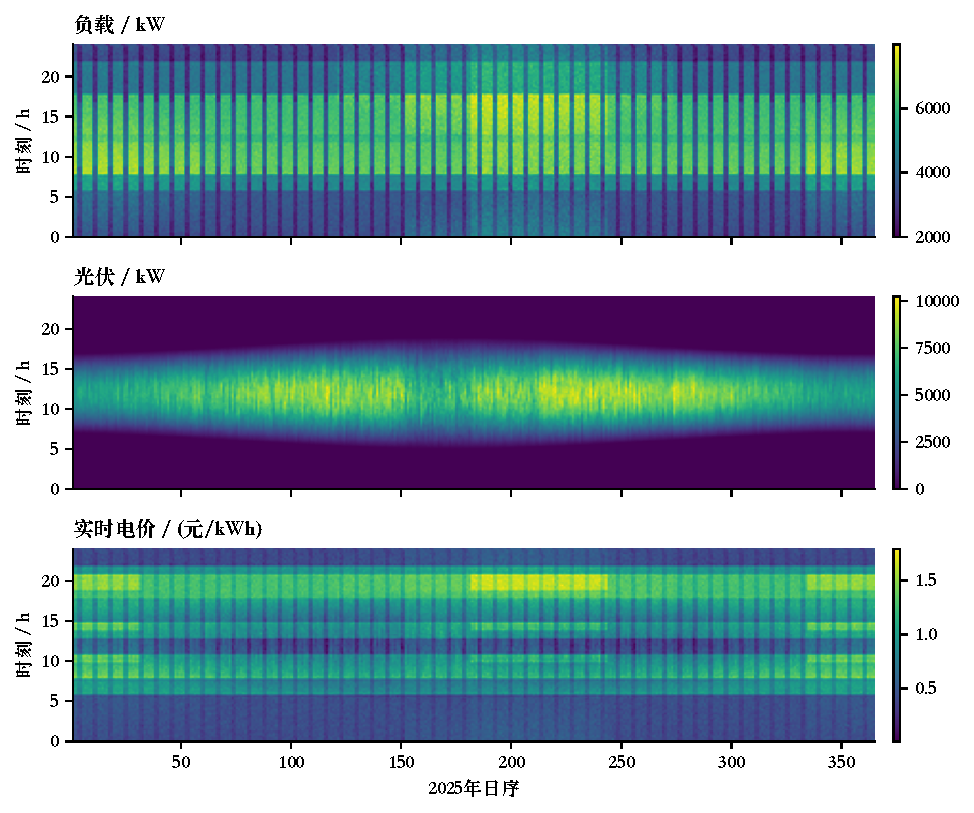
\includegraphics[width=0.86\linewidth]{figures/overview.pdf}
\caption{全年负载、光伏发电与实时电价的日内分布}\label{fig:overview}
\end{figure}

\subsection{符号说明与信息边界}
表\ref{tab:symbols}列出各问共用符号。带帽符号表示预测值，带横线符号表示优化得到的参考值，上标$\mathrm{act}$表示实际执行量。以$r$表示当前决策时刻，以$h$表示预测时域内的相对区间索引。
\begin{table}[htbp]\centering\small
\caption{主要符号及单位}\label{tab:symbols}
\begin{tabularx}{\linewidth}{lYl}\toprule
符号&含义&单位\\\midrule
$\ell_t,v_t,n_t$&负载电量、光伏电量、净负荷&kWh\\
$G_t^0,G_t$&午夜（零点）原计划购电量、经允许调整后的交付量&kWh\\
$X_t,W_t$&紧急购电量、无法利用的余电量&kWh\\
$C_t,D_t$&送入电池的充电量、由电池送出的放电量&kWh\\
$E_t$&第$t$段开始时电池内部储电量&kWh\\
$p_t,\widehat p_{t\mid r}$&实际结算价格、时刻$r$对$t$的预测价格&元/kWh\\
$\eta,B$&单程效率0.9、每段充放电上限$5000/6$&无量纲、kWh\\
$K,H_R,H_M$&可能情况的条数、长期与短期安排的区间数&条、段\\
$\bar C_t,\bar D_t,\bar E_t$&优化得到的参考充电、放电和储电量&kWh\\
$J^{\rm ref},C^{\rm act}$&预测条件下的目标值、实际支付费用&元\\\bottomrule
\end{tabularx}
\end{table}

\subsection{微网通用物理模型}
\subsubsection{微网能量流关系}
\begin{figure}[H]\centering
\includegraphics[width=0.85\linewidth]{../picture1.png}
\caption{微网能量流及储能调度关系}\label{fig:microgrid-flow}
\end{figure}

图\ref{fig:microgrid-flow}展示了微网各类电量的流向：光伏发电和计划购电共同满足小区负荷，剩余电量可充入电池以供后续时段使用；当两者与电池放电仍不足以覆盖负荷时，采用紧急购电补足缺口。未利用的余电不产生售电收入，且紧急购电仅用于满足负荷，不用于电池充电。

对任一区间，外网交付、紧急补购、光伏和电池放电是来源，负载、电池充电和弃置余电是去向，因此
\begin{align}
 G_t+X_t+v_t+D_t&=\ell_t+C_t+W_t,\qquad G_t,X_t,C_t,D_t,W_t\ge0,\label{eq:balance}\\
 E_{t+1}&=E_t+\eta C_t-D_t/\eta,\label{eq:soc}\\
 1200\le E_t&\le10800,\qquad 0\le C_t,D_t\le B=5000/6.\label{eq:bounds}
\end{align}
式\eqref{eq:balance}保证供电；式\eqref{eq:soc}记录充放电损耗；式\eqref{eq:bounds}保证储电量和功率不超限。100 kWh送入电池，只增加90 kWh储电量；从电池向外送出100 kWh，需要消耗$100/0.9$ kWh内部能量。

\subsubsection{通用约束表达}
由于余电$W_t$可以免费处置，只需在优化中保证供电不少于需要，即
\begin{equation}
 G_t+X_t+D_t-C_t\ge n_t.
 \label{eq:balance_ineq}
\end{equation}
求解完成后由式\eqref{eq:balance}计算余电。允许余电处置不等同于退还购电费，已承诺购电仍按规则结算。后续各问仅调整供需预测、购电调整权限与费用结构，通用物理约束保持不变。

\section{问题一模型的建立与求解}
\subsection{问题分析与建模思路}
问题一的144段负荷、光伏和电价均已知，是确定性多时段优化。储能把当前充放电与后续可用库存连接起来：若从低价时段购入1 kWh充电，经过两次效率损失后最多在高价时段送出$\eta^2=0.81$ kWh；光伏富余、功率上限和容量边界还会共同改变实际调度。目标与约束均为线性关系，故采用线性规划统一决定购电、充放电和储电状态。

\subsection{确定性优化模型}
沿用式\eqref{eq:balance_ineq}的供电条件及式\eqref{eq:soc}--\eqref{eq:bounds}的储能约束，问题一以$G_t,C_t,D_t$和区间起点储电量$E_t$为变量，不设置紧急购电。对$t=1,\ldots,144$，模型为
\begin{align}
 \min_{G,C,D,E}\quad&\sum_{t=1}^{144}p_tG_t,\label{eq:q1obj}\\
 \text{s.t.}\quad&G_t+D_t-C_t\ge n_t,\qquad G_t\ge0,\nonumber\\
 &E_{t+1}=E_t+\eta C_t-D_t/\eta,\nonumber\\
 &0\le C_t,D_t\le B,\qquad 1200\le E_t\le10800,\nonumber\\
 &1200\le E_{145}\le10800,\qquad E_1=E_{145}=6000.\label{eq:q1end}
\end{align}
供电约束的松弛量
\[
 W_t=G_t+D_t-C_t-n_t\ge0
\]
就是未被负载或电池利用的余电；它没有售电收入，也不会抵扣已经发生的购电费。终端等式则防止模型通过在最后时段耗尽原有电量得到不可重复的一次性低费用。

\subsection{充放电互斥性与求解方法}
上述目标和约束均为线性关系，属于凸优化中的线性规划\cite{boyd}。电池同段充、放电的直接约束$C_tD_t=0$是非线性的，但在本题允许免费处置余电的条件下，可以从任一同时充放电的可行解构造同费用的互斥解。

若$C_t,D_t>0$，令
\begin{equation}
 \delta_t=\min\{C_t,D_t/\eta^2\},\qquad
 C'_t=C_t-\delta_t,\qquad D'_t=D_t-\eta^2\delta_t.
 \label{eq:purify}
\end{equation}
变换后至少一个变量为零且功率上限仍成立，同时
\[
 \eta C'_t-D'_t/\eta=\eta C_t-D_t/\eta,\qquad
 D'_t-C'_t=D_t-C_t+(1-\eta^2)\delta_t.
\]
前式保证储电量轨迹不变，后式说明供电松弛只会增加；购电量$G_t$未变，故费用不增加。由此至少存在一个同段充放电互斥的最优解。若允许售电或出现负电价，则需重新检查这一结论。

程序使用HiGHS求解线性规划\cite{highs}，完成净化后重新回代全部物理约束；另求解带充放电状态变量的混合整数模型作独立核对。

\subsection{调度结果与运行规律}
最优全天购电量为59482.6990 kWh，购电费为35126.9486 元。图\ref{fig:dispatch}依次展示供需、储电量以及充放电功率与电价：购电不必逐段等于净负荷，电池在低价阶段和光伏富余阶段吸收电量，在较高电价阶段放电，最终回到6000 kWh。
\resultfigure[0.91]{dispatch}{问题一负载、光伏、购电、储电量及分时价格下的充放电轨迹}

表中指定10分钟区间按第\ref{sec:time-unit}节的自然日口径读取，例如12:00--12:10采用附件中12:10这一时刻的数据；完整144段结果写入\texttt{result1.xlsx}。充放电量均按电池外部计量，因而4小时储电量的净变化不等于该段“充电量减放电量”。
\sourceinput{tables_q1}
00:00--04:00累计充电4500.00 kWh、没有放电，电池内部增加4050.00 kWh；16:00--20:00累计放电5780.13 kWh，体现了跨时段转移。某个4小时汇总中充、放电量均为正，只表示不同10分钟区间先后发生充电和放电，不违反单段互斥。

\subsection{可行性与经济性检验}
将144段结果逐一代回能量平衡与储电量递推式，并与无储能基准$G_t=\max(n_t,0)$比较，得到表\ref{tab:q1-validation}。表中余电、残差和重叠量均由求解账本自动计算，而非在正文手工录入。
\begin{table}[H]\centering\small
\caption{问题一可行性与经济性检验}\label{tab:q1-validation}
\begin{tabular}{lrlr}\toprule
检验指标 & 数值 & 检验指标 & 数值 \\\midrule
无储能购电费/元 & 48052.05 & 优化后购电费/元 & 35126.95\\
节省费用/元 & 12925.10 & 相对节费率 & 26.90\%\\
最低储电量/kWh & 1200.00 & 最高储电量/kWh & 10800.00\\
24:00储电量/kWh & 6000.00 & 弃置余电/kWh & 0.00\\
最大能量平衡残差/kWh & $2.274\times10^{-13}$ & 最大储电量递推残差/kWh & $2.103\times10^{-12}$\\
最大同段充放电重叠/kWh & 0.00 & LP--MILP费用差/元 & 0.00\\\bottomrule
\end{tabular}\end{table}

与无储能方案相比，储能减少购电费\QOneSaving\ 元，节费率为\QOneSavingPct\%。储电量始终位于安全区间并准确恢复到初值，弃置余电在数值容差内为零；线性规划与强制互斥模型费用一致，支持上述互斥化处理和调度结果。
\FloatBarrier

\section{问题二模型的建立与求解}
\subsection{决策时序与两类模型框架}
问题二要求每天0时提交当日计划购电量，提交后不得回改；日内只能根据实际余缺调整储能动作，并以5倍价格补足最终缺口。为处理负载和光伏预测误差，本文在相同的物理约束和实际结算口径下构建两类方案：一类是“成本驱动的风险裕度日前规划—日内即时反馈控制模型”（简称“风险裕度—即时反馈模型”），用滚动残差分位数形成购电安全裕度；另一类是“12情境随机规划—4小时滚动控制模型”，用联合误差情境显式描述未来供需的不确定性。

两类模型是对不确定性和日内储能控制的两种处理路径。经相同评价期的回放比较，本文将费用和紧急购电表现更优的风险裕度—即时反馈模型作为问题二的最终方案，12情境模型则作为并列对照，并凭借其便于接入滚动预报和价格情境的结构，作为问题三、四的扩展基础。图\ref{fig:operation_timeline}具体表示风险裕度—即时反馈模型的信息流：前24小时计划正式提交，后24小时仅用于避免电池在日界处短视。
\begin{figure}[H]\centering
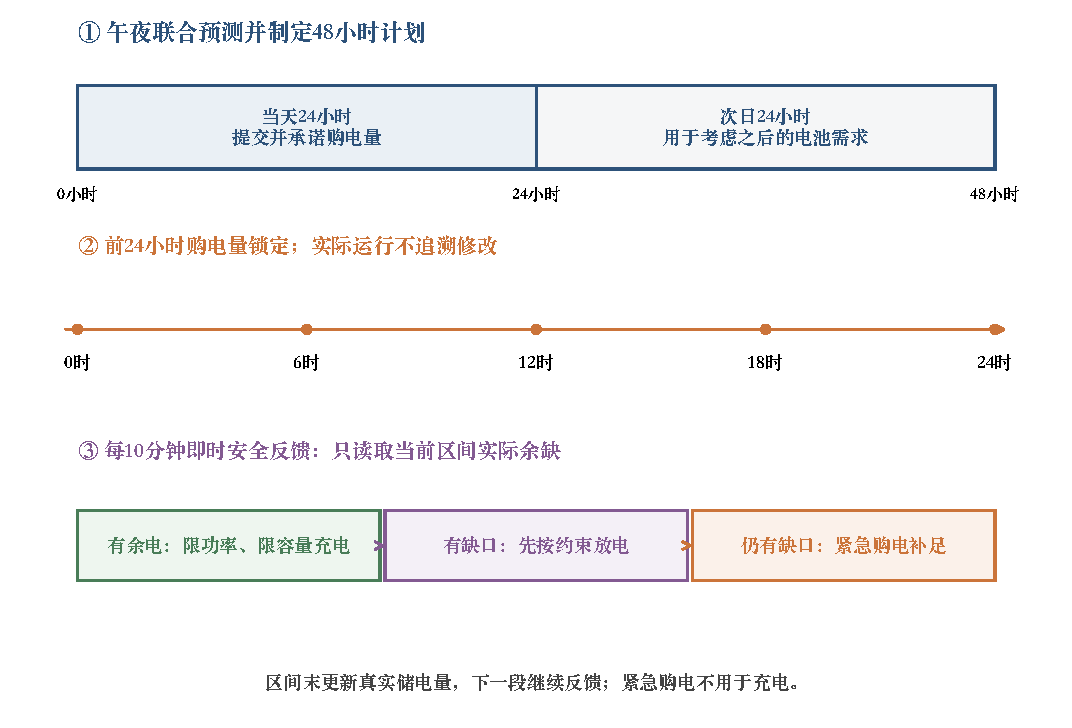
\includegraphics[width=0.93\linewidth]{figures/operation_timeline.pdf}
\caption{风险裕度—即时反馈模型的48小时计划与10分钟安全反馈}\label{fig:operation_timeline}
\end{figure}

全年从1月1日0时、储电量6000 kWh连续运行。1月既是历史逐步积累期，也是实际运行的预热期；2月1日不重置电池，正式334日直接继承1月末状态，这样避免人为选择有利初始储电量。

\subsection{联合因果预测与成本驱动的风险裕度}
对运行日$d$的负载和光伏，分别建立三个可解释基预测：前一日同段、前一周同段、最近7日逐段中位数。记其向量为$\bm b^L_{d,t},\bm b^V_{d,t}$，用此前最多14日数据求非负且和为1的权重：
\begin{equation}
 (\bm\alpha_d,\bm\beta_d)=\arg\min_{\bm\alpha,\bm\beta}
 \sum_{j=d-14}^{d-1}\sum_t\left|n_{j,t}-
 (\bm\alpha^\top\bm b^L_{j,t}-\bm\beta^\top\bm b^V_{j,t})\right|,
 \quad \bm1^\top\bm\alpha=\bm1^\top\bm\beta=1.
 \label{eq:q2weights}
\end{equation}
由此得到$\widehat\ell_{d,t}=\bm\alpha_d^\top\bm b^L_{d,t}$、$\widehat v_{d,t}=\bm\beta_d^\top\bm b^V_{d,t}$。历史不足7日时退化为前一日曲线，首日使用附件1；次日预测用当日预测值代替尚未发生的当日实测值，保证48小时计划严格因果。滚动训练和评价始终按时间顺序进行\cite{hyndman}。

记已揭晓净负荷残差为$e_{j,t}=n_{j,t}-(\widehat\ell_{j,t}-\widehat v_{j,t})$。从此前最多30日残差计算$q$分位数，并以“逐10分钟分位数”和“所在小时池化分位数”各50\%收缩，得到稳定裕度$m_{d,t}^{(q)}$；风险净负荷为
\begin{equation}
 N_{d,t}^{(q)}=\left[\widehat\ell_{d,t}-\widehat v_{d,t}+m_{d,t}^{(q)}\right]_+.
 \label{eq:risknet}
\end{equation}
分位数在评价前由题设价格关系确定。忽略储能考察单区间，若净负荷随机变量为$N$、计划购电为$G$，期望费用$f(G)=pG+5p\E[N-G]_+$。内点一阶条件为
\begin{equation}
 p-5p\Pr(N>G^*)=0,\qquad F_N(G^*)=0.8,
 \label{eq:quantile}
\end{equation}
故正式取$q=80\%$。这是一条事前风险折中依据，不是看完全年结果后挑选最便宜分位数。

\subsection{48小时计划购电模型}
每天0时单独求解一次48小时参考计划，并在该次求解内以$t=1,\ldots,288$作局部编号：$t=1$对应当天00:00--00:10，$t=145$对应次日00:00--00:10。将今、明两日的风险净负荷$N_t^{(0.8)}$拼接后，令$G_t,C_t,D_t,W_t$分别表示第$t$段内的计划购电量、充电量、放电量和未利用余电量，$E_t$表示第$t$段\emph{开始时}的储电量；$p_t$为该段电价。于是建立
\begin{align}
 \min\quad&\sum_{t=1}^{288}p_tG_t,\label{eq:q2plan}\\
 \text{s.t.}\quad&G_t+D_t-C_t-W_t=N_t^{(0.8)},\nonumber\\
 &E_{t+1}=E_t+\eta C_t-D_t/\eta,\nonumber\\
 &0\le C_t,D_t\le B,\quad W_t,G_t\ge0,\quad1200\le E_t\le10800,
 \qquad t=1,\ldots,288,\nonumber\\
 &E_1=E_0^{\rm act},\qquad E_{289}=6000.\label{eq:q2terminal}
\end{align}
其中，$E_0^{\rm act}$是当天0时从前序实际执行账本读出的已知储电量参数，$E_1$则是本次局部计划窗口第一段开始时的状态变量；等式$E_1=E_0^{\rm act}$将二者衔接。由递推式可知，$E_{145}$是前144段结束、即次日0时的储电量，$E_{288}$是最后一个10分钟区间开始时的储电量，而$E_{289}$才是288段全部执行后的48小时末端储电量。因此令$E_{289}=6000$ kWh，用于保留跨日库存价值，避免模型在最后一段透支电池；这不表示每天24时强制复位。

正式提交的仅是前144段（当天）的$G_t$；后144段仅作为跨日库存价值的参考，到次日0时会以新的历史信息和新的$E_0^{\rm act}$重新求解。模型为线性规划，可在全年逐日稳定求解。

\subsection{10分钟即时安全反馈}
对当前区间$r$，令$a_r=G_r+v_r-\ell_r$。若$a_r\ge0$，在功率与容量允许范围内尽量充电；若$a_r<0$，先放电，再用紧急购电补足：
\begin{align}
 C_r&=\min\{a_r,B,(10800-E_r)/\eta\},\qquad D_r=X_r=0,
 &&a_r\ge0,\nonumber\\
 D_r&=\min\{-a_r,B,\eta(E_r-1200)\},\quad X_r=-a_r-D_r,\quad C_r=0,
 &&a_r<0,\label{eq:q2feedback}\\
 W_r&=[a_r-C_r]_+,\qquad E_{r+1}=E_r+\eta C_r-D_r/\eta.\nonumber
\end{align}
该规则只读取本区间持续监测得到的平均供需，不回改$G_r$。它自动满足充放电互斥、禁止紧急购电充电，并把未满足负荷精确记入$X_r$。下一段从真实$E_{r+1}$继续，形成跨日连续闭环。

\subsection{风险裕度-即时反馈模型结果与敏感性}
问题二实际费用按
\begin{equation}
 C_2^{\rm act}=\sum_t p_tG_t+5\sum_t p_tX_t
 \label{eq:cost2}
\end{equation}
核算。正式334日总费用为\QTwoCost\ 元，其中计划费用\QTwoPlanCost 元、紧急购电费用\QTwoEmergencyCost 元；紧急购电量\QTwoEmergencyEnergy\ kWh。2月1日初始储电量为\QTwoInitialSOC kWh，年末为\QTwoFinalSOC kWh，均由1月连续运行和后续反馈自然得到。

表\ref{tab:q2-quantile}给出事前设定的70\%、80\%、90\%三组完整回放。80\%相对70\%仅增加\QTwoVsSeventyCostPct\%总费用，却使紧急购电量下降\QTwoVsSeventyEmergencyPct\%，在经济性与供电风险之间形成明显折中；90\%继续降低紧急量，但计划费用上升更多。因此，风险裕度—即时反馈模型采用由5倍紧急价格推导的80\%临界分位数，而不以事后最低总费用取代事前规则。
\sourceinput{q2_sensitivity}

\subsection{12情境随机规划与4小时滚动控制模型}
该方案的核心思路是把问题二分成“\textbf{日前定合同、日内调储能、实时保供电}”三个层次。每日0时，48小时情境规划同时权衡普通购电费和不同供需情境下的紧急购电风险，只将前24小时的购电量作为不可更改的当日合同；进入日内后，每10分钟根据最新历史和真实库存重算未来4小时的储能轨迹，但只执行第一个10分钟动作；本区间供需实现后，再由安全层修正该动作并计算紧急购电。三层的作用如表\ref{tab:q2-scenario-timing}所示。

\begin{table}[H]\centering\small
\caption{12情境方案的决策时序与各层作用}\label{tab:q2-scenario-timing}
\begin{tabularx}{\linewidth}{p{2.1cm}p{2.2cm}YY}\toprule
层次&求解时刻&主要输入与输出&实际采用部分\\\midrule
日前规划&每日0时&由当时可得历史构造12条未来路径，得到购电计划及参考储能轨迹&提交前24小时购电量；后24小时只作为跨日参考\\
日内控制&每10分钟开始前&读取当前真实储电量，在固定购电合同下重算未来24段充放电轨迹&只采用首段充、放电目标，下一段重新求解\\
安全执行&供需实现后&用实际负载、光伏和设备边界修正首段目标&有余电才充电，有缺口才放电，仍不足时紧急购电\\\bottomrule
\end{tabularx}
\end{table}

\subsubsection{负载--光伏联合情境}
在任一决策时刻$r$，先以同星期历史、近期均值和附件1先验形成未来基准预测$\widehat\ell_{r+h\mid r}$、$\widehat v_{r+h\mid r}$。再从决策时刻以前最多60日中选取$K=12$个已经完整揭晓的连续误差块；第$k$个块同时提供负载误差$\varepsilon_{h}^{L,k}$和光伏误差$\varepsilon_{h}^{V,k}$，由此构造
\begin{equation}
 \ell_{r+h}^{(k)}=\bigl[\widehat\ell_{r+h\mid r}+\varepsilon_h^{L,k}\bigr]_+,
 \qquad
 v_{r+h}^{(k)}=\bigl[\widehat v_{r+h\mid r}+\varepsilon_h^{V,k}\bigr]_+,
 \qquad
 n_{r+h}^{(k)}=\ell_{r+h}^{(k)}-v_{r+h}^{(k)}.
 \label{eq:q2scenario-generation}
\end{equation}
同一情境中的两类误差取自同一历史起点，且保留整段误差序列，不逐时打乱，因而能够同时保留负载与光伏的相关性以及误差的时间连续性。12条情境等权使用；所有误差块均在$r$之前完整结束，因此模型不会读取决策时尚未发生的数据。每日0时规划取$H_R=288$段，日内控制取$H_M=24$段，分别对应48小时和4小时。

\subsubsection{第一层：每日0时的48小时情境规划}
在本次48小时窗口内，以$t=1,\ldots,H_R$作局部编号。$G_t$为计划购电量，$\bar C_t,\bar D_t,\bar E_t$为参考充电量、放电量和储电量；$X_t^{(k)},W_t^{(k)}$分别为情境$k$下可能需要的紧急购电量和未利用余电量。模型为
\begin{align}
 \min\quad
 &\sum_{t=1}^{H_R}p_tG_t
 +\frac1K\sum_{k=1}^{K}\sum_{t=1}^{H_R}5p_tX_t^{(k)},\label{eq:q2reference}\\
 \text{s.t.}\quad
 &G_t+X_t^{(k)}+\bar D_t-\bar C_t-W_t^{(k)}=n_t^{(k)},
 &&t=1,\ldots,H_R,\ k=1,\ldots,K,\nonumber\\
 &\bar E_{t+1}=\bar E_t+\eta\bar C_t-\bar D_t/\eta,
 &&t=1,\ldots,H_R,\nonumber\\
 &0\le \bar C_t,\bar D_t\le B,\quad G_t\ge0,
 &&t=1,\ldots,H_R,\nonumber\\
 &1200\le\bar E_t\le10800,
 &&t=1,\ldots,H_R+1,\nonumber\\
 &X_t^{(k)},W_t^{(k)}\ge0,
 &&t=1,\ldots,H_R,\ k=1,\ldots,K,\nonumber\\
 &\bar E_1=E_0^{\rm act},\qquad \bar E_{H_R+1}=6000.\nonumber
\end{align}
目标函数第一项是确定支付的计划购电费，第二项是12条等概率路径下的平均紧急购电费。关键在于，$G_t,\bar C_t,\bar D_t,\bar E_t$对所有情境均相同，表示在未来误差尚未揭晓时就要给出一条共同的计划；只有$X_t^{(k)}$和$W_t^{(k)}$随情境变化，用来核算不同路径下可能出现的缺电和余电。因此，模型不会利用“提前知道将发生哪条情境”的信息来选择储能动作。

48小时末端的6000 kWh只用于防止有限时域模型在末端透支电池，并不要求每天24时恢复到6000 kWh。求解后仅提交$t=1,\ldots,144$的$G_t$，次日部分和整条$\bar E_t$均为日内控制提供参考；下一日0时仍从实际库存重新规划。

\subsubsection{第二层：固定合同下的4小时滚动控制}
设$r$为当前10分钟区间的开始时刻。此时当日购电合同$G$已经确定，不能因新预测而修改。记$\widetilde G_{r+h}$为本次4小时控制窗口内固定使用的购电量：位于当日的区间采用已提交合同，若窗口跨到次日，则采用午夜规划中尚未提交的次日参考值。模型以实际库存$E_r^{\rm act}$为起点，重新构造未来$H_M=24$段的12条联合情境，求解共享的充放电轨迹$\bar C_{r,h}^{M},\bar D_{r,h}^{M},\bar E_{r,h}^{M}$：
\begin{align}
 \min\quad
 &\frac1K\sum_{k=1}^{K}\sum_{h=0}^{H_M-1}5p_{r+h}X_{r,h}^{(k)},\label{eq:q2mpc}\\
 \text{s.t.}\quad
 &\widetilde G_{r+h}+X_{r,h}^{(k)}+\bar D_{r,h}^{M}-\bar C_{r,h}^{M}-W_{r,h}^{(k)}
 =n_{r+h}^{(k)},\nonumber\\
 &\bar E_{r,h+1}^{M}=\bar E_{r,h}^{M}
 +\eta\bar C_{r,h}^{M}-\bar D_{r,h}^{M}/\eta,\qquad
 \bar E_{r,0}^{M}=E_r^{\rm act},\nonumber\\
 &\bar E_{r,H_M}^{M}=E_r^{\rm tar},
 \quad 0\le\bar C_{r,h}^{M},\bar D_{r,h}^{M}\le B,
 \quad1200\le\bar E_{r,h}^{M}\le10800,\nonumber\\
 &X_{r,h}^{(k)},W_{r,h}^{(k)}\ge0,
 \qquad h=0,\ldots,H_M-1,\ k=1,\ldots,K.\nonumber
\end{align}
式\eqref{eq:q2mpc}中没有再写计划购电费，是因为$\widetilde G_{r+h}$在本次求解中已固定，该项对储能决策是常数；此时优化的目的，就是利用电池尽量降低未来4小时的期望紧急购电费。

短窗口末端目标取自48小时参考轨迹。若实际库存已经偏离参考轨迹，原目标可能在4小时内无法到达，因此先按功率与容量限制投影：
\begin{align}
 L_r&=\max\{1200,E_r^{\rm act}-H_MB/\eta\},\qquad
 U_r=\min\{10800,E_r^{\rm act}+H_MB\eta\},\nonumber\\
 E_r^{\rm tar}&=\min\{U_r,\max\{L_r,\bar E_{r+H_M}^{48}\}\}.
 \label{eq:q2mpc-terminal}
\end{align}
其中$\bar E_{r+H_M}^{48}$是午夜48小时规划给出的同一时刻参考库存。投影使末端约束位于当前库存理论上可达的区间内，从而避免短窗口因库存偏差而不可行。每次求解后只取$h=0$的$\bar C_{r,0}^{M},\bar D_{r,0}^{M}$作为本区间目标；到$r+1$时读入新的实际库存并重复上述过程，这就是4小时滚动控制。

\subsubsection{第三层：按实际供需安全执行}
滚动优化使用的是预测情境，不能直接保证首步目标一定符合本区间的实际余缺。令$a_r=G_r+v_r-\ell_r$，则安全层执行
\begin{align}
 C_r^{\rm act}&=\min\left\{\bar C_{r,0}^{M},[a_r]_+,B,
 \frac{10800-E_r^{\rm act}}{\eta}\right\},\nonumber\\
 D_r^{\rm act}&=\min\left\{\bar D_{r,0}^{M},[-a_r]_+,B,
 \eta(E_r^{\rm act}-1200)\right\},\nonumber\\
 X_r^{\rm act}&=[-a_r-D_r^{\rm act}]_+,\qquad
 W_r^{\rm act}=[a_r-C_r^{\rm act}]_+,\nonumber\\
 E_{r+1}^{\rm act}&=E_r^{\rm act}+\eta C_r^{\rm act}-D_r^{\rm act}/\eta.
 \label{eq:q2scenario-execution}
\end{align}
因此，实际有余电时才允许充电，实际有缺口时才允许放电，放电后仍未满足的负荷才由紧急购电补足。该规则保证紧急购电不会用于充电，并使实际能量平衡、功率限制和储电量边界始终成立。需要特别区分：48小时规划决定当日购电合同，4小时模型只给出储能目标，安全层才产生最终实际充放电量与紧急购电量。

\subsubsection{结果比较}
12情境模型属于有限情境随机规划与滚动控制的结合\cite{shapiro,rawlings,parisio}。其334日实际总费用为\QTwoReferenceCost 元，紧急购电量为\QTwoReferenceEmergencyEnergy{} kWh。相同设备参数、评价日期和结算口径下，风险裕度—即时反馈模型少支出\QTwoReferenceSaving 元，即\QTwoReferenceSavingPct\%；紧急购电量减少\QTwoReferenceEmergencySaving{} kWh，即\QTwoReferenceEmergencySavingPct\%，因此本文选其作为问题二最终方案。

这一结果表明，在本年度数据和题设5倍紧急购电价格下，12条等权历史情境对高净负荷尾部的覆盖仍然有限；直接用80\%分位数形成合同安全裕度，实际回放表现更好。该结论是同一数据集上的模型比较，并不意味着分位数模型在其他年份或其他应急价格下必然占优。12情境模型能够保留联合误差路径，且便于在新预报到达后重构未来情境，因此仍作为问题三、四的扩展基础；其参数、逐时账本和复现入口均保留在支撑材料中。

\subsection{指定日期结果与可行性}
以下四个日期的计划购电、充放电、储电量和紧急购电均由风险裕度—即时反馈模型账本自动聚合。6月21日光伏充足，实际电费最低；12月21日净负荷较高，实际电费最高。四日中只有9月23日发生紧急购电，集中在20:20--20:30且仅6.38 kWh，说明80\%裕度覆盖了绝大多数展示日偏差，但仍保留少量尾部缺口。
\sourceinput{tables_q2}
\sourceinput{day_interpretations_q2}
全年逐段验证能量守恒、储电量递推、容量与功率边界、跨日连续、充放电互斥、禁止紧急购电充电及训练信息边界；检验结果见第\ref{sec:validation}节。
\FloatBarrier

\section{问题三模型的建立与求解}
\subsection{模型选择依据与总体思路}
问题三的难点是新信息分批到达，而每次只能修改尚未执行的合同；购电调整、储能库存和紧急补购又通过未来供需共同耦合。单点滚动优化会忽略尾部误差，完整多阶段情景树则随信息节点迅速膨胀。因此，本文采用\textbf{12情境随机规划与4小时滚动控制}：预报发布时重构联合误差路径并优化未执行合同，发布时点之间每10分钟重算储能轨迹、只执行首步，最后由安全层保证实际供电。该结构保留误差相关性和时间连续性，又能把分段线性调整费用直接纳入线性规划\cite{shapiro,rawlings,parisio}。

$K=12$与4小时窗口由计算量和收益共同确定：情境数由6增至12可降低17.78万元，继续增至24仅再降低4.10万元；控制窗口由2小时增至4小时降低2.32万元，继续增至6小时仅再降低0.99万元。问题三的预报价值只与同一模型下“仅0时预报”比较，避免把更换模型的影响误认为新预报收益。

\subsection{调整机制与决策变量}
问题三在上述框架中引入6时、12时和18时发布的新光伏预报，并据此调整尚未执行的购电计划。购电量的调整方向由最新预报、附件1规定的标准购电价格及调整结算规则共同决定：当预计缺电风险上升时，可上调计划购电量，以减少价格更高的紧急购电；当预计净需求下降时，则可下调计划购电量，从而减少部分原计划费用。

每日0时，模型利用当时最新发布的光伏预报制定日前购电计划$G^0$；在其余预报发布时点，仅对当前及后续尚未交付区间的有效购电量$G$进行调整。购电计划仅在规定的预报发布时点更新，储能决策则以10分钟为间隔执行，因此二者具有不同的决策时间尺度。各版预报严格按照其发布时间纳入模型，并仅在相应的24小时预测范围内进行插值；超出该范围的时段仍采用历史预测结果。

\subsection{调整费用与上下调边际}
令$a_t^+=\left[G_t-G_t^0\right]_+$为上调量，$a_t^-=\left[G_t^0-G_t\right]_+$为下调量。实际电费为
\begin{equation}
 C_3^{\rm act}=\sum_t p_t\left(G_t^0-0.5a_t^-+1.5a_t^++5X_t^{\rm act}\right).
 \label{eq:cost3}
\end{equation}
式中四项依次表示原计划费用、取消部分对应的费用扣减、新增购电费用和紧急购电费用。该结算方式也可表述为：下调时，保留量$G_t$按标准购电价格支付，取消量$G_t^0-G_t$按$0.5p_t$支付违约费用；上调时，原计划量按标准购电价格支付，新增量按$1.5p_t$支付。对每个时段，仅按照最终生效购电量与午夜原计划之间的差额结算一次，不累计计算历次调整产生的中间差额。

例如，设标准购电价格为1元/kWh，午夜原计划购电量为100 kWh。上调至120 kWh时，计划及调整费用为$100+1.5\times20=130$元；下调至80 kWh时，保留的80 kWh支付80元，取消的20 kWh按50\%支付10元，合计$80+0.5\times20=90$元。这也等于$100-0.5\times20$元。

按照上述结算规则，每下调1 kWh购电量可节省$0.5p_t$，因此优化模型不应预先排除下调决策。为说明上下调决策的边际条件，暂不考虑储能，并以$N$表示随机净需求。当$G<G^0$时，增加1 kWh计划购电量的边际费用为$0.5p_t$，与其减少缺电风险所带来的$5p_t\Pr(N>G)$相平衡，对应净需求的90\%分位数；当$G>G^0$时，边际费用为$1.5p_t$，对应净需求的70\%分位数。因此，在单时段情形下，当$G^0$低于净需求的70\%分位数时，应上调购电量；当其高于90\%分位数时，应下调购电量；当其位于二者之间时，则维持原计划不变。全年模型还包含储能及其跨时段耦合关系，实际调整方案由完整优化模型求得。

\subsection{滚动调整优化模型}
每次新预报发布后，模型首先更新未来光伏预测及其对应的12种误差情景，随后以当前实际储电量为初始状态，重新求解后续时域的购电与储能计划。记$\mathcal A_r$为当日尚未执行的时间区间集合，$\mathcal B_r$为次日的参考时间区间集合，则滚动优化目标为
\begin{align}
 \min\quad J_3(r)={}&
 \sum_{t\in\mathcal A_r}p_t(G_t^0-0.5a_t^-+1.5a_t^+)
 +\sum_{t\in\mathcal B_r}p_tG_t\nonumber\\
 &+\frac1K\sum_{k=1}^K\sum_{t\in\mathcal A_r\cup\mathcal B_r}5p_tX_t^{(k)}.
 \label{eq:updateobj}
\end{align}
模型保留情景供电约束、储电量递推关系和全部设备运行限制，并对当日尚未执行的区间增加以下约束：
\[
 G_t-G_t^0=a_t^+-a_t^-,\qquad a_t^+,a_t^-\ge0,\qquad t\in\mathcal A_r.
\]

优化以$E_r^{\rm act}$为起点，并将48小时参考时域的末端储电量保持为6000 kWh。由于次日购电计划尚未提交，因此$\mathcal B_r$中的购电量仅按附件1规定的标准购电价格参与参考优化；待次日0时，再重新生成该日的正式购电计划。

求解完成后，模型使用新的$G$替换尚未执行区间的原购电计划，而已经发生的购电行为及相应费用保持不变。问题三沿用12情境模型的4小时滚动优化机制和安全执行规则。由此，新预报不仅能够改变后续时段的有效购电计划，还会影响储能在不同时段之间的能量配置。

\subsection{预报发布时点选择}
为识别不同日内预报更新的边际作用，本文设置五种方案：仅使用0时预报；在0时预报的基础上，分别增加6时、12时或18时的一次更新；以及采用6时、12时和18时的全部更新。各方案采用相同的设备参数、预测基线、结算规则和评价日期，仅改变允许使用的预报发布时点。

正式评价期内，仅使用0时预报时的总费用为\QThreeIssueZeroCost 元；采用全部三次日内更新后降至\QThreeCost 元，共节省\QThreeUpdateSaving 元，即\QThreeSavingPct\%。在三种单次更新方案中，增加6时、12时和18时更新后的费用分别为\QThreeIssueSixCost 元、\QThreeIssueTwelveCost 元和\QThreeIssueEighteenCost 元，其中12时更新收益最大；在0时和12时更新基础上采用全部更新，还可减少\QThreeAllVsTwelveSaving 元。因此，本文将全部日内更新方案作为问题三主策略。

日内预报更新主要通过三种途径降低运行费用：第一，当预计缺电风险上升时，以1.5倍标准购电价格上调计划购电量，从而减少按5倍标准购电价格结算的紧急购电；第二，当预计供电余量增加时，下调计划购电量；第三，根据光伏预测的变化重新优化后续储能轨迹。当预报发布时间较晚或储电量达到边界时，更新所带来的边际收益可能较小。相关研究同样强调，应以最终调度成本评价预测结果的改进\cite{mazzola}。

\subsection{策略比较与结果分析}
问题三在正式评价期内的费用为\QThreeCost\ 元，紧急购电量为\QThreeEmergencyEnergy\ kWh。其严格控制组为同一模型中仅使用0时预报的方案；全部日内更新相对该控制组节省\QThreeUpdateSaving 元，即\QThreeSavingPct\%，并使紧急购电量减少\QThreeEmergencySaving\ kWh，即\QThreeEmergencySavingPct\%。因此，新预报的价值不仅体现为更低的合同费用，也体现为对高价缺口的及时修正。

从调整方向看，334天内累计上调\QThreeAdjustmentUpWan 万 kWh、下调\QThreeAdjustmentDownWan 万 kWh，最终有效购电量较午夜计划净减少\QThreeAdjustmentNetDownWan 万 kWh。下调量明显大于上调量，说明日内信息主要用于撤回偏保守的日前承诺；但选择性上调仍不可缺少，它以1.5倍价格替代了部分5倍紧急购电。单次更新中12时费用最低，表明接近日间光伏峰值的新信息最有价值；全部三次更新仍优于只在12时更新，说明早晚偏差也会通过储能库存影响后续费用。

需要说明的是，问题二最终采用的风险裕度—即时反馈模型与问题三采用的12情境滚动框架在误差处理和日内控制方式上不同，因此二者的费用差异不能直接归因于预报更新。问题三的预报信息价值应通过本节设置的内部控制实验进行评价；跨问题的结果仅在统一运行汇总表中并列展示，不能替代问题三内部方案之间的比较。

\texttt{result3.xlsx}分别记录零点原计划、调整后的最终有效购电量以及储能的实际运行情况。下文选取与问题二相同的四个指定日期展示调度结果，以便在统一的数据口径下进行对照。
\sourceinput{tables_q3}
\sourceinput{day_interpretations_q3}
\FloatBarrier

\section{问题四模型的建立与求解}
\subsection{电价预测与实际结算}
问题四在问题二和问题三的基础上进一步考虑实时电价的变化。由于制定购电计划时无法提前获得未来的真实电价，因此需要根据已经发生的历史电价对未来价格进行预测。

对于未来各时段的电价，本文利用过去28天中相同星期的电价均值、最近7天的电价均值以及附件1电价，分别赋予$0.60$、$0.30$和$0.10$的权重，得到基础预测\cite{lago}：

\[
\hat p_t^{\,\mathrm{base}}
=
0.60p_t^{\,\mathrm{week}}
+
0.30p_t^{\,\mathrm{recent}}
+
0.10p_t^{\,\mathrm{prior}},
\]

其中，$p_t^{\,\mathrm{week}}$表示近期相同星期对应时段的历史电价，$p_t^{\,\mathrm{recent}}$表示最近7天对应时段的平均电价，$p_t^{\,\mathrm{prior}}$表示附件1给出的参考电价。

再用决策时刻以前的历史误差修正基础值，得到$\hat p_{r+h|r}$，并构造$K$条可能价格路径。第$k$种情景下

\[
p_{r+h}^{(k)}
=
\exp
\left(
\log \hat p_{r+h|r}
+
\varepsilon_{h}^{\log p,k}
\right),
\]

其中$\varepsilon_{h}^{\log p,k}$为第$k$个历史块中的对数价格误差。本文取$K=12$，且负载、光伏和电价误差来自同一段历史，使每条情景保留三者的共同变化；实际电价始终只用于交付结算和事后评价。

\subsection{两类交易机制的统一模型}
先用一个费用系数$g_t$表示普通购电及调整部分：尚可自由安排购电的区间取$g_t=G_t$；问题三式的当天调整区间取$g_t=G_t^0-0.5a_t^-+1.5a_t^+$。波动电价下的长计划目标统一为
\begin{equation}
 \min\quad J_4=\frac1K\sum_{k=1}^K\sum_t
          p_t^{(k)}\bigl(g_t+5X_t^{(k)}\bigr).
 \label{eq:q4}
\end{equation}
不允许日内调整时，午夜确定当天$G^0$后不再改变；允许调整时，在规定发布时刻按问题三的原计划基准更新$G$。供电、储能、末端和执行规则均与各自对应的固定电价方案一致，区别是目标中的价格也随情景变化。短期4小时控制同样用对应价格情景计算平均应急费用。

实际结算仍分别采用式\eqref{eq:cost2}和式\eqref{eq:cost3}，其中$p_t$取交付区间真实价格。预测价格仅用于决策，实际价格用于结算，二者对应的目标值与实付费用严格区分。

\subsection{运行结果与策略比较}
对334天连续回放，不允许日内调整时总费用为\QFourTwoCost\ 元、紧急购电量为\QFourTwoEmergencyEnergy\ kWh；允许调整后分别降至\QFourThreeCost\ 元和\QFourThreeEmergencyEnergy\ kWh。后者节省\QFourSaving\ 元，即\QFourSavingPct\%，并减少紧急购电\QFourEmergencySaving\ kWh，即\QFourEmergencySavingPct\%。允许调整策略的有效购电量较仅零点计划净减少\QFourAdjustmentNetDown\ kWh，说明波动价格下日内更新同样主要用于撤回不再经济的承诺，同时通过选择性上调控制高价缺口。

在允许调整的模型内部，全部更新较仅0时预报节省\QFourUpdateSaving\ 元，即\QFourUpdateSavingPct\%。另设“提前知道未来真实电价、供需仍按因果预测”的信息对照：不允许和允许调整两种策略分别仅再节省\QFourTwoKnownPriceSaving\ 元和\QFourThreeKnownPriceSaving\ 元，比例为\QFourTwoKnownPriceSavingPct\%和\QFourThreeKnownPriceSavingPct\%。这表明在本年度数据中，价格预测改进仍有价值，但收益小于储能和日内供需信息带来的改善。

然而，提前知道真实电价后，紧急购电量并不一定减少。这是因为模型可能选择在部分低价时段减少提前购电，而在必要时通过紧急购电补足需求。只要其他购电费用的下降幅度大于紧急购电费用的增加，总费用仍可能降低。因此，评价调度策略时应以最终总费用为主要指标，而不能只比较紧急购电量。

附录进一步给出同时已知未来供需与价格且放宽交易收费的全年下界，用于刻画理论改进空间。两组完整结果分别写入 result4-2.xlsx 和result4-3.xlsx。以下保留题目要求的四个日期及全部指定时段；图\ref{fig:costs}进一步比较四种主策略的费用组成与累计费用。
\sourceinput{tables_q4_2}
\sourceinput{tables_q4_3}
\sourceinput{day_interpretations_q4}
\resultfigure{costs}{334天内四种主策略的实际费用组成与累计费用}
\FloatBarrier

\section{模型检验与结果分析}\label{sec:validation}

\subsection{物理可行性检验}

求解器得到最优解后，还需要检查结果是否满足能量平衡和储能运行约束。为此，对每个时段分别计算能量平衡误差和储电量变化误差：

\[
r_t^{\mathrm{bal}}
=
G_t+X_t+v_t+D_t-\ell_t-C_t-W_t,
\]

\[
r_t^{\mathrm{soc}}
=
E_{t+1}-E_t-\eta C_t+\frac{D_t}{\eta}.
\]

若模型运行正确，上述两个误差都应接近于0。同时检查储电量是否处于规定范围内、充放电功率是否超过上限、是否出现同一时段同时充放电，以及紧急购电是否被用于电池充电。

检验结果表明，各方案均满足上述要求。所有结果中最大能量平衡误差为
$2.274\times10^{-13}\,\mathrm{kWh}$，最大储电量变化误差为
$2.104\times10^{-12}\,\mathrm{kWh}$，均可认为接近于0；同时未出现储能越界、功率超限和同一时段同时充放电等情况。因此，模型计算结果满足实际运行的基本约束。


\subsection{储电量差异与费用比较}

不同策略在评价期结束时可能具有不同的剩余储电量。如果只比较已经支付的电费，可能会出现某个方案通过大量消耗原有储能而表现出较低费用的情况。

因此，在比较不同策略时，除报告实际费用外，进一步对期初和期末储电量差异进行统一校正：

\[
\lambda
=
\frac{\min_t p_t^{(\text{附件1})}}{0.9},
\]

\[
C_{\mathrm{inv}}
=
C_{\mathrm{act}}
+
\lambda(E_{\mathrm{start}}-E_{\mathrm{end}}).
\]

其中，$C_{\mathrm{act}}$ 为实际运行费用，
$E_{\mathrm{start}}$ 和 $E_{\mathrm{end}}$ 分别表示评价期开始和结束时的储电量。
该校正值仅用于不同策略之间的公平比较，不计入题目要求的实际购电费用。

进一步对每日费用差进行重复抽样，计算平均节省费用的 $95\%$ 区间。结果表明，问题二主模型、问题三采用全部预报更新以及问题四允许日内调整三种改进方案，其平均节省费用的区间下限均大于0，说明这些改进在本年度数据上均表现出较稳定的节费效果。


\subsection{敏感性分析}

为判断模型中的主要设置是否合理，分别改变部分条件并重新计算，包括去除储能、使用单一预测代替12种情景、改变情景数量、改变光伏预报更新时间以及调整滚动控制时间范围等。

结果表明，四种主策略相对各自无储能方案均节费\StorageSavingMinPct\%--\StorageSavingMaxPct\%，说明跨时段储能是节省开支的重要方法。问题二取消预测安全裕度后，总费用由\QTwoCostWan 万元上升至\QTwoNoMarginCostWan 万元，表明仅围绕平均预测签订合同会显著增加高价紧急购电。

同时，对情景数量、控制时长和预报更新时间进行调整后，模型总体结论没有发生明显改变，说明所建立的购电与储能调度策略具有一定的稳定性。

此外，本文还对储能效率和购电调整费用的不同理解进行了重新计算。结果表明，这些参数和交易规则会对最终费用产生一定影响，因此在实际应用中应根据具体设备参数和交易规则重新确定模型参数。

主要比较结果汇总如下。全部33组实验的原始费用、紧急电量和储电量校正结果放入附录\ref{app:technical}。这些实验用于检查结论，不用正式334天的结果事后重选风险裕度的分位数参数。
\sourceinput{validation}
\resultfigure{ablation}{问题三及其波动价格版本中，不同预报更新组合相对完整更新的实际费用变化}
\FloatBarrier

\section{结论与模型评价}

\subsection{主要结论}
四问结果形成一条清晰主线：确定信息下，储能通过低价与光伏富余充电、高价放电获得主要节费；供需未知时，由5倍紧急价格导出的80\%分位数在计划费和缺电风险间给出事前折中；日内预报到达后，调整主要撤回偏保守合同，同时以少量上调替代昂贵补购；价格波动下，评价标准仍是含计划、调整和紧急费用的实际总成本，而非单独追求最少紧急电量。全过程回放、控制实验和统计区间共同支持这些结论。

\subsection{优点、限制与改进}
模型以同一能量账本贯通四问，严格区分计划、参考轨迹和实际动作，并把因果预测、合同结算与设备约束落实到每个10分钟区间；五个工作簿和33组实验均可由程序独立复算。

局限主要有四点：问题二即时反馈按当前余缺贪心充放电，可能未把电量保留给未来更高价格或更大缺口；固定80\%分位数在极端天气下未必合适；12条历史情景不能覆盖全部尾部事件；10分钟平均模型未考虑电池退化、线路容量和更短时标响应。后续可采用随季节和天气变化的分位数、带终端价值的自适应反馈、更丰富的情景缩减，并用多年度数据检验泛化能力。上述改进需要新增数据或设备参数，不能由本年度样本内回看替代。

\section*{AI工具使用声明}
本参赛队在竞赛过程中使用了AI工具，主要用于资料检索、模型讨论、代码辅助、结果核验和论文表述优化，详细使用情况见支撑材料。

\begingroup\small\setstretch{1.0}\raggedright\interlinepenalty=10000
\bibliographystyle{unsrtnat}
\bibliography{references}
\endgroup
\label{LastMainPage}
\clearpage
\appendix
\ctexset{
  section={name={附录,：},number=\Alph{section}},
  subsection={number=\Alph{section}.\arabic{subsection}},
  subsubsection={number=\Alph{section}.\arabic{subsection}.\arabic{subsubsection}}
}
\section{支撑材料文件说明}
\noindent 本页列出支撑包中的全部文件及用途。支撑包仅保留可运行建模代码、题目要求的结果文件与AI工具使用详情；题目原始附件不重复打包。全部文件均采用匿名名称，路径相对于支撑包根目录。
\begin{center}\small
\begin{tabularx}{\linewidth}{>{\raggedright\arraybackslash}p{0.43\linewidth}Y}\toprule
文件或目录&内容和用途\\\midrule
\texttt{README.md}&支撑材料文件列表、数据放置、环境与执行命令\\
\texttt{requirements.txt}&Python依赖及固定版本\\
\texttt{run.py}&问题一至问题四、结果导出与核验的统一入口\\
\texttt{src/microgrid/}&数据、预测、优化、仿真、导出与核验的9个完整Python源文件\\
五个\texttt{result*.xlsx}&题目指定的全部结果工作簿，位于支撑包根目录\\
AI工具使用详情.pdf&AI名称、用途、提示过程、采纳与核验范围\\\bottomrule
\end{tabularx}
\end{center}
\noindent\textbf{题目要求的结果文件：}\texttt{result1.xlsx}、\texttt{result2.xlsx}、\texttt{result3.xlsx}、\texttt{result4-2.xlsx}、\texttt{result4-3.xlsx}。问题一结果覆盖144段；其余文件覆盖2月1日至12月31日334天，储能结果为实际动作与实际储电量。

\noindent\textbf{复算顺序：}按README将官方附件置于\texttt{C题/附件/}，安装依赖后依次执行\texttt{q1}、\texttt{calibrate}、\texttt{select}、\texttt{main}、\texttt{export --results-only}和\texttt{verify --require-workbooks}。计算产生的逐时账本、校准记录与核验文件属于本地中间文件，不放入提交包。后续附录先给技术细节和完整实验表，再列全部自编程序。本轮AI差异须由队员据实复核。
\clearpage
\section{技术补充与复现细节}
\label{app:technical}
\label{app:implementation}

本附录说明正文模型如何转换为可重复执行的计算过程。公式中的计划购电量$G_t^0,G_t$、充放电量$C_t,D_t$、紧急购电量$X_t$及余电量$W_t$均为10分钟区间的交流侧电量，储电量记为$E_t$；单向效率为$\eta=0.9$。完整程序紧接本附录列出，运行顺序与依赖版本见支撑材料\texttt{README.md}。

\subsection{问题二风险裕度—即时反馈模型的实现}
问题二正式入口为\texttt{simulate\_quantile\_q2}。每天只拟合一次预测权重：前一日、前一周和最近7日中位数构成三列基预测，最近14日内全部10分钟样本共同最小化净负荷绝对误差；负载权重和光伏权重分别非负且和为1。历史不足8日时采用前一日曲线，首日采用附件1。最近30日已揭晓净负荷残差用于计算70\%、80\%或90\%分位数；逐段分位数与同小时池化分位数各取一半。次日预测以当日预测代替未揭晓的当日实际曲线，故48小时输入不含未来实测值。

48小时稀疏线性规划以计划购电费为目标，固定起点真实储电量和末端6000 kWh，仅提交前144段。日内每10分钟直接按当前实际余缺执行：余量为正时充到功率或容量边界，余量为负时先放到功率或储电下界，仍有缺口才记紧急购电；不调用另一个MPC函数。配置字段\texttt{model=rolling\_quantile}、\texttt{feedback=immediate\_safe}和\texttt{control\_hours=0}共同标识该正式路径。

70\%、90\%、无分位数裕度和无储能方案均使用同一实现，只改变一个预先声明的参数。作为并列候选的12情境随机规划方案由\texttt{scenario\_reference}独立运行，其预测审计与逐日结果置于\texttt{q2\_model\_comparisons/}；完整逐时账本可由同一入口重建。

\subsection{12情境模型及问题三、四的预测与情景生成}
\label{app:forecast}

\paragraph{26维特征构造。}
为说明特征的时间关系，令$D$为本次午夜预测的日序号，$a$为目标日序号，$s=0,\ldots,143$为日内区间。把三个预测目标写为
\begin{equation}
 z_{a,s}=(L_{a,s},V_{a,s},\log p_{a,s})^{\mathsf T},\qquad
 A=\operatorname{diag}(5000,5000,1).
\end{equation}
其中$L,V$单位为kW，$A$用于统一残差的数值尺度。朴素预测的负载、光伏基线见正文；对数价格基线依次以$0.60,0.30,0.10$加权过去28天同星期均值、最近7天均值和附件1先验。历史不足时取已有天数；无同星期样本时改用最近样本；首日直接使用附件1。

每个目标区间的输入$x_{D,a,s}$含四组各3维的曲线特征：基线、起点前最近完整日、目标日的7天滞后、附件1先验，均左乘$A^{-1}$。最近完整日固定为$D-1$；只有$0\le a-7<D$时才取实际7天滞后，否则使用先验。其余14维为
\begin{equation}
 (\sin\theta_s,\cos\theta_s,\sin2\theta_s,\cos2\theta_s,
   \sin\phi_a,\cos\phi_a,a-D,\text{目标星期的7维独热编码}),
\end{equation}
其中$\theta_s=2\pi(s+1)/144$，$\phi_a=2\pi a/365.25$。
独热编码是以一个1和六个0表示星期类别。预测次日时，最近日特征仍取$D-1$，不会改取尚未结束的$D$日。固定电价问题在全部特征和残差计算中使用附件1日价格曲线；附件4实际价格仅进入问题四。

\paragraph{岭回归与梯度提升残差校正。}
设训练目标为$y_i=A^{-1}(z_i-\widehat z_i^{\rm base})$，以$y_i^{\mathsf T}$为行组成矩阵$Y$，列向量$\mu_Y$记录三个目标的训练均值。岭回归先用训练样本均值和标准差标准化$X$，标准差小于$10^{-12}$的列以1替代除数，再求解
\begin{align}
 \widehat W&=\arg\min_W\left\|Y-\bm1\mu_Y^{\mathsf T}-X_{\rm std}W\right\|_F^2
                       +30\|W\|_F^2,\\
 \widehat z&=\widehat z^{\rm base}+A(\mu_Y+\widehat W^{\mathsf T}x_{\rm std}).
\end{align}
截距不受惩罚。实现求解加上$30I$的正规方程，并检查系数有限性。

提升树分别拟合三个残差目标。以某一目标为例，从训练均值$F_0$开始，用回归树逐轮拟合尚未解释的残差：
\begin{equation}
 F_m(x)=F_{m-1}(x)+0.08\,g_m(x),\qquad m=1,\ldots,60.
\end{equation}
对于给定的树分区，记所拟合目标的残差为$y_i^{\ast}$，叶值对应平方损失与L2惩罚
$\frac12\sum_i\{y_i^{\ast}-F_{m-1}(x_i)-g_m(x_i)\}^2+\frac52\sum_j b_j^2$，
其中$b_j$为叶节点的输出；分裂由直方图算法搜索。固定最多15个叶节点、每叶最少36个样本、L2参数5，随机种子2026，关闭早停。树的输出同样乘回$A$并加到基线上。

\paragraph{滚动训练与预测缓存。}
在第$D$日，训练样本的历史预测起点依次取$\max(1,D-60),\ldots,D-1$，每个起点生成本日及次日目标，但仅保留目标日严格小于$D$的样本。这样，训练用到的实际结果均来自已经结束的完整日。岭回归保留全部144个日内点；提升树在拼接后的训练序列上每隔一个点取样，预测仍覆盖全部144个点。少于7天历史时，两种复杂模型均退回朴素基线。

基础模型每日拟合一次，并由同一午夜起点生成本日、次日及第三日共432步预测；第三日沿用同一模型和已知日历特征。这份缓存足以覆盖日内任一时刻发出的最长48小时查询。训练提前日数只有0和1，因此跨到第三日的部分是模型外推。每10分钟控制更新实际库存，使用当前已发布的光伏预报；基础负载和价格模型不在日内反复重训。

\paragraph{官方预报融合与历史误差块。}
每次只取允许发布时刻中最新且已经发布的一版光伏预报。其24个点对齐到发布时间后的第1至24小时，以最近已结束区间的实测光伏为插值锚点，形成10分钟预测；首个起点没有实测时使用附件1末点。超出该版预报覆盖范围后使用历史模型。消融实验中，未列入该实验的发布时刻对预测和购电调整同时不可用。

令当前绝对区间起点为$r=144D+s$，预测长度为$H$。历史块起点取$j=144d+s$，其中
\begin{equation}
 \max(0,D-60)\le d<D,\qquad j+H\le r.
\end{equation}
后一条件保证块内$H$个实际区间全部结束。历史基线取第$d$日原始午夜生成的完整三日预测，再截取$s$起的$H$步；若使用官方预报，则只叠加在历史起点$j$已经发布的版本。三条误差序列为负载和光伏的加性误差、价格的对数误差，按同一历史块配对，按正文情景公式转换为净负荷电量与正价格。

把合格块按时间排序，取等距索引$\operatorname{round}(\operatorname{linspace}(0,M-1,K))$，其中$M$为合格块数。12情境模型及问题三、四取$K=12$，等权使用选中的块；$M<K$时允许重复，无合格块时使用零残差。点预测消融$K=1$单独规定为零残差。若2月启动的模型尚无自己的1月预测记录，就在各历史起点严格重建朴素预测，并标记为因果朴素初始化；不会用2月拟合的模型回填1月预测。

\paragraph{模型选择与数值保护。}
12情境模型及问题三、四的三个候选各自从1月1日6000 kWh开始假想运行，以1月15日至31日的库存校正费用选模。它们1月15日的库存可以不同，比较时保存各自期初、期末值。具体规则是在费用不超过候选最小值的$1.005$倍的模型中，依朴素、岭回归、提升树的顺序取最简单者。其正式1月始终按朴素策略预热，2月继承该实际库存；候选实验不会改写这段运行。问题二风险裕度—即时反馈模型不使用这套选模结果。

负载和光伏预测截到非负区间。进入对数的价格设置$10^{-6}$下限；点预测和情景预测的对数价格在指数变换前截到$[-9,3]$，即价格约束于$[1.23\times10^{-4},20.09]$元/kWh。此界远宽于附件4的正常取值范围，用于防止外推造成数值溢出。任何非有限预测或回归系数均触发异常，不以替换结果的方式继续运行。

\subsection{参考末端、数值恢复与实际运行记录}
\label{app:records}

\paragraph{末端库存可达域。}
正文的短时域末端目标来自48小时参考轨迹。若实际库存偏离参考，原目标可能无法在剩余$H_M$步内达到，因此先将它投影到
\begin{equation}
 \left[\max\{1200,E_r-H_MB/\eta\},
       \min\{10800,E_r+H_MB\eta\}\right],\qquad B=5000/6\ \mathrm{kWh}.
\end{equation}
区间两端分别对应持续最大功率放电和充电，考虑了容量、功率与效率。投影后作为本次参考优化的硬末端条件。它只表达设备的库存可达性；实际安全层还受当期余电和缺口限制，可能无法跟踪参考末端，下一步应从实际$E$重新规划。2小时控制窗口更短，投影对避免功率限制导致的不可行尤为必要。本段只适用于12情境模型及问题三、四，不适用于问题二风险裕度—即时反馈模型。

\paragraph{求解结果数值复核。}
稀疏线性规划调用HiGHS，原始及对偶可行性容差均为$10^{-8}$；混合整数核验的相对间隙设为$10^{-8}$。程序要求求解状态为最优，并执行正文所述的同充同放消除，再由$C,D$重算整条$E$、各情景$X,W$及目标值。恢复后的参考约束最大偏差不得超过$2\times10^{-5}$，重算目标与求解器目标的差不得超过
$10^{-4}+10^{-7}\max\{1,|J_{\rm raw}|\}$。
这一步验证的是参考问题，实际电费仍由逐区间执行和结算产生。输入库存仅允许在边界外$10^{-7}$的舍入范围内截回容量界，更大越界直接报错。

\paragraph{运行记录内容。}
工程中，每个策略的\texttt{ledger.npz}保存全年逐区间数组，其字段含义如下。所有电量字段以kWh计，价格为元/kWh，费用为元。
\begin{center}
\small
\begin{tabularx}{\linewidth}{p{0.22\linewidth}Y}
\toprule
记录内容 & 字段与含义\\
\midrule
交易和实际供需 & \texttt{plan}为$G^0$，\texttt{effective}为$G$；\texttt{load,pv,price}为结算区间的实际负载电量、光伏电量和价格。\\
储能和补缺 & \texttt{charge,discharge,emergency,waste}对应$C,D,X,W$；\texttt{soc\_start,soc\_end}为两端$E$。\\
费用分项 & \texttt{base\_fee,up\_fee,down\_fee,emergency\_fee}记录原计划费、最终上调费、最终下调费、应急费；\texttt{cost}为其和。\\
控制和预测摘要 & 情景模型中\texttt{target\_charge,target\_discharge}为安全层执行前的首步建议；问题二风险裕度—即时反馈模型中二者记录即时反馈实际值。\texttt{expected\_net,expected\_price}为执行前参考预测；\texttt{issue\_index}为最近承诺更新时间。\\
\bottomrule
\end{tabularx}
\end{center}
\texttt{revisions.json.gz}记录每次调整时刻及调整后的剩余日承诺向量，保存到小数点后9位。\texttt{forecast\_diagnostics.json}保存日级训练审计、调用次数及冷启动记录数；\texttt{summary.json}保存策略配置和分评价窗口汇总。审计字段\texttt{training\_\allowbreak actual\_\allowbreak end\_\allowbreak exclusive}是可用历史的排他上界：索引达到该值的区间尚不能用于训练。\texttt{issue\_index}也不等于每次预测所用的完整预报元数据。

提交包将五种策略的完整账本保存为\texttt{q1\_ledger.npz}至\texttt{q4\_3\_ledger.npz}。各数组按10分钟顺序排列，首项对应2025年1月1日00:00--00:10；该格式保留全部字段并减少压缩包体积。提交包中的调整记录与预测审计也加相同策略前缀并以gzip压缩，例如\texttt{q2\_revisions.json.gz}与\texttt{q2\_forecast\_diagnostics.json.gz}。

\paragraph{在线检查与独立复核。}
预测返回时检查历史误差块结束位置不晚于当前起点、预报发布时间不晚于当前时刻。执行时即时检查库存边界、能量平衡及充放电与应急充电重叠；独立验证程序再从实际账本重算守恒、库存连续、功率界、安全层动作和各费用分项，物理容差为$10^{-6}$ kWh。工作簿另按原模板日期、时段及单元格逐项核对，连续应急区间先展开再与账本比较。

程序未保存全年每次预测的完整情景及全部信息元数据，也未持久化每次线性规划的完整目标记录。因此，信息边界结论由实现约束、即时断言、日级审计和测试共同支持；保存的账本足以重算实际物理量与电费，不能单独复原所有中间预测。真实组件的3日端到端测试将同一历史前缀后的负载、光伏、价格及尚未发布预报共同扰动，检查此前的计划、储能建议、实际库存和费用不变。指定日期的LP/MILP对照则是使用已实现净负荷的事后数值核验，不参与过去的运行决策。

\subsection{统计口径与信息下界}
\label{app:statistics}

\paragraph{预测评价指标口径。}
午夜24小时预测对正式期334天的全部日内点计算负载、光伏及价格MAE；问题二账本保存午夜联合预测，情景模型的每10分钟首步预测由账本中的情景均值计算净负荷电量及价格MAE、RMSE。附件3原始预报按发布时间与提前1至24小时分别统计，只使用实际光伏大于100 kW且存在实测的白天目标。后者剔除跨入2026年的无实测点。三者的提前量、样本与单位不同，图中的白天预报误差不能代替整日能量误差；光伏大量零值也使全时段MAPE不适合作为主要指标。

\paragraph{库存校正与配对区间估计。}
评价费用$C$之外，以固定$\lambda=\min p^{(\text{附件1})}/0.9$计算
$C^{\rm inv}=C+\lambda(E_{\rm start}-E_{\rm end})$。
两端库存同时计入，适用于正式期和1月候选比较；该校正不进入题目要求的实际电费。比较两种策略的日费用时，先按相同日期求差$\delta_d=C_d^{\text{前者}}-C_d^{\text{后者}}$，再做循环区块重采样：每次均匀抽取$\lceil334/7\rceil=48$个起点，各带连续7日并在序列末尾循环，拼接后截到334日。固定种子2026，重复2000次，取样本日均差的2.5\%和97.5\%分位数。正值表示后者节省，负值表示后者更贵。循环处理和单年季节性限制了区间的外推能力，该区间用于描述本年差异。

\paragraph{未来信息对照实验。}
仅价格全知实验用真实未来价格替换评价年内的预测价格，净负荷预测、参考结构及安全层保持原配置；超出2025年的参考部分仍使用预测价。它检验价格信息在这套近似策略中的作用，费用不必单调下降。

完全信息下界使用全年365天真实净负荷与相应真实价格，所有购电按基础价计费，初始$E=6000$，末端只受容量界约束。令其购电变量为$g_t$，保留相同储能物理约束并满足$g_t+v_t+D_t\ge\ell_t+C_t$。任一主结算实际策略都能取$g_t=G_t+X_t$形成可行解，且
\begin{equation}
 C-\sum_t p_t(G_t+X_t)
 =\sum_t p_t\left[\tfrac12(G_t-G_t^0)^+
                  +\tfrac12(G_t^0-G_t)^++4X_t\right]\ge0.
\end{equation}
因此该放松规划的最优值不超过相同全年范围的主策略费用。差额同时包含未来信息、交易限制和控制近似的影响；它不能与334日费用直接相减，也不能全部视为可实现的节省。

\subsection{校准、预测诊断与完整实验表}
\label{app:experiments}
下表保留候选校准和各变体的原始数值。33组实验包括问题二的无储能、无分位数裕度、70\%、90\%和12情境模型5组，问题三与问题四的点预测、储能、更新时点、情景数、控制时域、效率与结算解释等28组。参数变体分别运行并按自己的效率及结算条款核验；主参数和事前规则不因正式期结果而改变。
\begin{table}[H]\centering\small\caption{情景滚动模型一月后半月预测方法选择（储电量校正后的费用，元）}
\begin{tabular}{lrrrl}\toprule
策略 & 季节朴素 & 岭回归 & 梯度提升 & 入选方法\\\midrule
问题二12情境模型 & 993038.99 & 1021829.62 & 1007275.41 & 季节朴素\\
问题三 & 974841.35 & 994073.34 & 973691.02 & 季节朴素\\
问题四-2 & 1146794.67 & 1199761.83 & 1177412.12 & 季节朴素\\
问题四-3 & 1107397.57 & 1139949.50 & 1121541.43 & 季节朴素\\
\bottomrule\end{tabular}\end{table}
\begin{table}[H]\centering\small\caption{午夜对当天24小时的平均绝对预测误差}
\begin{tabular}{lrrr}\toprule
策略 & 负荷/kW & 光伏/kW & 电价/(元/kWh)\\\midrule
问题二 & 181.34 & 156.59 & 0.000000\\
问题三 & 282.38 & 197.49 & 0.000000\\
问题四-2 & 282.38 & 167.60 & 0.050916\\
问题四-3 & 282.38 & 197.49 & 0.050916\\
\bottomrule\end{tabular}\end{table}
{\small\begin{longtable}{lrrr}
\caption{33组对照与参数检验完整结果（二月至十二月）}\\\toprule
策略变体 & 实际费用/万元 & 紧急量/MWh & 库存校正费用/万元\\\midrule\endfirsthead
\caption[]{33组对照与参数检验完整结果（续）}\\\toprule
策略变体 & 实际费用/万元 & 紧急量/MWh & 库存校正费用/万元\\\midrule\endhead
问题二：无分位数裕度 & 1510.36 & 315.31 & 1510.37\\
问题二：无储能 & 1859.39 & 258.47 & 1859.39\\
问题二：70\%分位数 & 1456.17 & 136.19 & 1456.19\\
问题二：90\%分位数 & 1495.52 & 36.52 & 1495.55\\
问题二：12情境随机规划模型 & 1482.49 & 253.92 & 1482.52\\
问题三：原计划全额另加违约费 & 1484.12 & 165.99 & 1484.14\\
问题三：2小时 & 1468.53 & 178.81 & 1468.54\\
问题三：6小时 & 1465.22 & 180.46 & 1465.26\\
问题三：仅0时 & 1505.78 & 243.13 & 1505.81\\
问题三：0、12时 & 1474.24 & 197.08 & 1474.26\\
问题三：0、18时 & 1494.55 & 217.10 & 1494.57\\
问题三：0、6时 & 1489.54 & 198.05 & 1489.56\\
问题三：24情景 & 1462.12 & 171.67 & 1462.15\\
问题三：6情景 & 1483.99 & 223.53 & 1484.00\\
问题三：无储能 & 1897.66 & 257.66 & 1897.66\\
问题三：点预测 & 1624.09 & 833.48 & 1624.09\\
问题三：往返效率90\% & 1419.29 & 177.16 & 1419.33\\
问题四-2：价格全知 & 1540.94 & 267.45 & 1540.93\\
问题四-2：无储能 & 1973.43 & 319.20 & 1973.43\\
问题四-2：点预测 & 1869.85 & 1192.80 & 1869.82\\
问题四-3：原计划全额另加违约费 & 1557.73 & 163.61 & 1557.67\\
问题四-3：2小时 & 1539.54 & 176.11 & 1539.48\\
问题四-3：6小时 & 1538.07 & 177.72 & 1538.02\\
问题四-3：仅0时 & 1581.84 & 243.03 & 1581.78\\
问题四-3：0、12时 & 1547.26 & 194.42 & 1547.20\\
问题四-3：0、18时 & 1570.00 & 216.90 & 1569.95\\
问题四-3：0、6时 & 1563.37 & 196.79 & 1563.32\\
问题四-3：24情景 & 1529.55 & 169.15 & 1529.54\\
问题四-3：6情景 & 1562.38 & 219.05 & 1562.33\\
问题四-3：价格全知 & 1523.23 & 192.97 & 1523.22\\
问题四-3：无储能 & 1965.48 & 256.10 & 1965.48\\
问题四-3：点预测 & 1719.17 & 849.87 & 1719.15\\
问题四-3：往返效率90\% & 1491.10 & 172.31 & 1491.04\\
\bottomrule\end{longtable}}
逐时独立验证的最大能量平衡误差为$2.274\times 10^{-13}$ kWh；问题一LP与MILP费用差为0.000000000元。
全年365日完全信息松弛下界：固定电价13751266.38元，波动电价14494771.23元。该下界允许年末自由储电，与334日表内费用不能直接相减。
对应365日实际费用：问题二16757631.12元，问题三16684412.30元，波动电价下分别为18076656.90元、17650372.98元。差额同时包含信息、交易限制和策略近似的影响。
\resultfigure{forecast}{附件3光伏预报的平均绝对误差随提前小时数变化：正式334日，仅取实际光伏大于100 kW的时段}
\resultfigure{sensitivity}{情景数、控制范围及费用解释变化时，实际费用相对主策略的变化}
\FloatBarrier


\clearpage
\sourceinput{appendix}
\end{document}
